\documentclass[12pt,pdftex]{article}
\usepackage[pdftex]{graphicx,color}
\usepackage{setspace,palatino,multirow}
\usepackage{amsmath,amssymb}
\usepackage{titlesec}
\usepackage{lscape}
%\usepackage{subfigure}
\usepackage{threeparttable}
\usepackage{natbib}
\bibliographystyle{ecta}
\usepackage{cite}
\usepackage{booktabs}
\usepackage{subcaption}
\usepackage{pdflscape}
\usepackage{afterpage}
\usepackage{xcolor}
\usepackage{rotating}

\definecolor{nblue}{RGB}{0,0,128}

\usepackage[pdftex,colorlinks=true, bookmarks=false,
pdfstartview={XYZ null null 0.65},
pdftitle={},
pdfauthor={ Michael E. Waugh},
pdfkeywords={},
colorlinks=true,linkcolor=darkgray,citecolor=darkgray,urlcolor=darkgray,
breaklinks]{hyperref}

\newcounter{saveeqni}%
\newcounter{saveeqn01i}%
\newcommand{\alpheqni}{\setcounter{saveeqni}{\value{section}}%
%\setcounter{saveeqn01i}{\value{subsectioni}}%
\renewcommand{\theequation}
    {\alph{saveeqni}\mbox{.\arabic{equation}}}}%
\newcommand{\reseteqni}{\setcounter{equation}{\value{saveeqni}}%
\renewcommand{\theequation}{\arabic{equation}}}%

\newtheorem{as}{Assumption}
\newtheorem{reg}{Regularity Condition}
\newtheorem{conjecture}{Conjecture}
\newtheorem{corr}{Corollary}
\newtheorem{df}{Definition}
\newtheorem{lemma}{Lemma}
\newtheorem{prp}{Proposition}
\newtheorem{rmk}{Remark}
\newenvironment{prf}{{\bf Proof}}{\hfill { }}
\newtheorem{proposition}{Proposition}

\DeclareMathOperator*{\plim}{plim}
\DeclareMathOperator*{\umax}{max}

\special{papersize=8.5in,11in}
\onehalfspacing
\setlength{\parindent}{0.1em}
\setlength{\parskip}{.09in}
\textwidth15.75cm
\evensidemargin 1.5in
\oddsidemargin 1.5in
\topmargin 8.5cm
\textheight 10in
\hyphenation{over-lapping}

\titleformat{\section}{\color{black}\large\bf}{\color{black}{\thesection.}}{.25cm}{}
\titleformat{\subsection}{\color{black}\normalsize\bf}{\thesubsection.}{.5em}{}
\titleformat{\subsubsection}{\color{black}\normalsize\bf}{\thesubsubsection.}{.5em}{}

\titlespacing{\section}{0pt}{*1.5}{*.5}
\titlespacing{\subsection}{0pt}{*1.5}{*.5}
\titlespacing{\subsubsection}{0pt}{*1.5}{*.5}

\def\thesection{\arabic{section}}
\def\thesubsection{\arabic{section}.\arabic{subsection}}
\def\thesubsubsection{\arabic{section}.\arabic{subsection}.\Alph{subsubsection}}

\def\citeapos#1{\citeauthor{#1}'s (\citeyear{#1})}

\renewcommand{\arraystretch}{1.1}
\usepackage[margin=2cm]{geometry}

\begin{document}
\begin{onehalfspacing}
\newpage

\normalsize



\section{Rural Urban Migration and the Efficient Allocation}\label{sed:intro}

This section solves and computes the efficient allocation in our model economy. Up to this point, we have measured the welfare gains from a particular policy intervention|a subsidy to induce more seasonal migration. In all the instances we studied (one-time partial equilibrium, permanent general equilibrium with distortionary taxes) the welfare gains from these interventions result from the provision of an opportunity to that allows households to better smooth their consumption by moving across space.

However, all these experiments leave open the normative question about and how much households \emph{should} migrate when markets are complete and the economy is undistorted. In other words, what is the first-best allocation and how does it compare to the aforementioned policy interventions? This is what we study below.

\subsection{The Social Welfare Function}

To study these normative questions, we take a stand on the social welfare function. We focus on a utilitarian planner placing equal weight on households. Define the social welfare function as
\begin{align}
\mathcal{W^{SP}} = \sum_{t=0}^{\infty}\sum_{j} \int\limits_{z} \int\limits_{s} \int\limits_{x} \int\limits_{\nu} \beta^{t} \ u_{j}(c_{j}(z, s, x, t), x, \nu) \lambda_{j}(z, s, x, \nu, t) dz \ ds \ dx \ d\nu.
\label{eq:sp-social_welfare}
\end{align}
Here social welfare is the average value of households utility across locations $j$, productivity states $z$ and $s$, experience $x$, and preference shocks $\nu$. The average is computed with respect to the measure of households $\lambda_{j}(z, s, x, \nu, t)$ with those shock states, experience levels, and preference shocks at date all dates $t$. Utility depends directly upon the consumption allocation $c_{j}(z, s, x, t)$, but also  directly on the location $j$ through the $\bar u$, and the idiosyncratic preference shock.

We cast the Planners Problem in terms of the planner choosing consumption allocations and migration probabilities. To cast the problem in terms of migration probabilities, we integrate out the preference shocks conditional on a set of migration probabilities for each household state. These migration probabilities prescribe an assignment of those households with the largest relative preference shock to migrate or not. So given set of states $j, z, s, x, t$, utility is
\begin{align}
u(c_{j}(z,s, x, t), x) + E[ \ \nu \ | \ \big\{\mu_{j',j}(z,s,x,t)\big\}_{j'} ].
\label{eq:utility-shocks}
\end{align}
where $\mu_{j',j}(z,s,x,t)$ is the migration probability going from location $j$ to location $j'$ and then $E[ \ \nu \ | \ \big\{\mu_{j',j}(z,s,x,t)\big\}_{j'} ]$ is the expected value of the preference shock conditional on the migration probabilities. So, for example, if all people migrate location $j$ to location $j'$, then this value is just the unconditional mean of a Type 1 extreme value shock. Now we can write the social welfare function as
\begin{align}
\mathcal{W^{SP}} = \sum_{t=0}^{\infty}\sum_{j} \int\limits_{z} \int\limits_{s} \int\limits_{x} \beta^{t} \bigg \{ u(c_{j}(s, x, t), x) + E[ \ \nu \ | \ \big\{\mu_{j',j}(s,x,t)\big\}_{j'}] \bigg \} \lambda_{j}(s, x, t) dz \ ds \ dx.
\label{eq:sp-social_welfare2}
\end{align}

\subsection{The Law of Motion and Feasibility}

The Planning Problem maximizes (\ref{eq:sp-social_welfare2}) subject to the law of motion describing how the population evolves across states and locations and then how many resources the are available, i.e., feasibility. We describe each of these aspects of the environment below.

\textbf{Law of Motion.} The law of motion describing how the measure of households evolves across states and locations is
\begin{align}
\lambda_{j}(z, s', x', t+1)  & =  \int\limits_{s} \int\limits_{x}  \mu_{j,j}(z, s,x,t)\pi(s',s) \varphi(x',x, j) \lambda_{j}(z, s, x, t)  \ ds \ dx  \  \label{eq:planner_law_motion} \\
& +  \sum_{j' \neq j} \int\limits_{s} \int\limits_{x} \mu_{j,j'}(z, s,x,t) \pi(s',s) \varphi(x',x, j') \lambda_{j'}(z, s, x, t)  \ ds  \ dx. \nonumber
\end{align}
where $\pi(s',s)$ describes the transition across transitory states and $\varphi(x',x, j')$ describes the transition in experience. This equation says, given the current distribution $\lambda_{j'}(z, s, x, t)$ in location $j'$, the measure of households $\lambda_{j}(z, s', x', t+1)$ reflects the migration probabilities of households in each location (the $\mu$'s), how their productivity evolves over time ($\pi's$), and how their experience $\varphi(x',x, j)$ evolves.

\textbf{Labor Supply, Aggregate Production, and the Resource Constraint.} Given a distribution of households, the effective labor units in the urban and rural area are
\begin{align}
N_{u,t} =& \sum_{j = [\mbox{\tiny urban}, \mbox{\tiny seas}]}\int\limits_{z} \int\limits_{s} \int\limits_{x} \  z s^{\gamma} \ \lambda_j(z, s, x, t) \ dz \ ds \ dx, \nonumber
\\
\nonumber \\
N_{r,t} =& \int\limits_{z} \int\limits_{s} \int\limits_{x} \ s \ \lambda_{\mbox{\tiny rural}}(z, s, x, t)\ dz \ ds \ dx \ .
\label{eq:planner_labor_supply}
\end{align}
with the urban area includes the seasonal and permanent urban workforce. Aggregate production of the final good is
\begin{align}
Y_t = A_u N_{u,t} + A_{r,t} \left(N_{r,t} \right)^{\phi}.
\label{eq:planner_value_production}
\end{align}
Combining the amount of resources available in (\ref{eq:planner_value_production}) with the consumption and moving decisions we have the following resource constraint:
\begin{align}
Y_t\  \geq \ & \sum_{j} \int\limits_{z} \int\limits_{s} \int\limits_{x} c_{j}(z, s, x, t) \lambda_{j}(z, s, x, t) \ dz \ ds \ dx  \nonumber \\
& \ \ \ \ +  \ \  \sum_{j}\sum_{j'} \int\limits_{z} \int\limits_{s} \int\limits_{x}  m_{j',j} \ \mu_{j',j}(z,s, x, t) \lambda_{j}(z, s, x, t) \ dz \ ds \ dx.
\label{eq:planner_income_side_gdp}
\end{align}
which says that production must be greater than or equal to consumption which is the first term on the righthand side of (\ref{eq:planner_income_side_gdp}) and the moving costs associated with the migration of households across locations which is the second term on the righthand side. Here we compactly sum across all $j'$ and $j$ location pairs with the notion that the moving cost for staying in a location is zero, i.e., $m_{j,j} = 0$.

\subsection{The Planner's Problem and the Efficient Allocation}

The Planner chosees consumption allocations and migration probabilities to maximize the social welfare function in (\ref{eq:sp-social_welfare2}) subject to the constraints imposed by feasibility (\ref{eq:planner_income_side_gdp}), the law of motion (\ref{eq:planner_law_motion}), and that the migration probabilities sum to one. In math, the problem is
\begin{align}
\small
& \max \ \sum_{t=0}^{\infty}\sum_{j} \int\limits_{z} \int\limits_{s} \int\limits_{x} \beta^{t} \bigg \{ u(c_{j}(z, s, x, t), x) + E[\ \nu \ | \ \mu_{j',j}(z, s,x,t)] \bigg \} \lambda_{j}(z, s, x, t) \ dz \ ds \ dx \label{eq:planner_problem} \\
& \mbox{subject to} \nonumber\\[.75em]
& \ \ \ \ \mbox{feasibility}, \ \ (\ref{eq:planner_income_side_gdp}), \ \ \ \ [\ \mathbf{\chi(t)} \ ], \nonumber \\[.75em]
& \ \ \ \ \mbox{law of motion}, \ \ (\ref{eq:planner_law_motion}), \ \ \ \ [\ \mathbf{\chi_{3j}(s, x, t)} \ ], \nonumber \\[.75em]
& \ \ \ \ \mbox{migration probabilities}, \ \ \sum_{j'} \mu_{j',j}(s,x,t) = 1,  \ \ \ \ [\ \mathbf{\chi_{2j}(s, x, t} \ ], \nonumber \\[.75em]
& \ \ \ \ \mbox{and an inital condition}, \ \ \ \ \lambda_j(s, x,0). \nonumber
\end{align}
where the $\chi$ terms in brackets denote the Lagrange Multipliers associated with constrained optimization problem. We the call the allocation induced by the solution to \ref{eq:planner_problem} as the \emph{efficient allocation}. After deriving the necessary conditions associated with \ref{eq:planner_problem}, Proposition \ref{prp:efficient} characterizes the consumption allocations and migration probabilities associated with these necessary conditions.

\begin{proposition}[\textbf{Efficient Consumption and Migration}] \label{prp:efficient} The consumption and migration rates that solving the Planners Problem in (\ref{eq:planner_problem}) are: Consumption allocations equate the marginal utility of consumption in all locations, productivity and experience states for each date $t$:
{\small
\begin{align}
u'(t) = u'(c_{j}(z, s, x, t)) = u'(c_{j'}(z, s', x', t)) \ \forall \ j, \ z, \ s, \ x, \ \mbox{and}  \ j', \ s', \ x'.
\label{eq:foc_planner2}
\end{align}
}
Migration probabilities satisfy
{\footnotesize
\begin{align}
& \mu_{j'j}(z,s,x,t)  =  \exp \left(\frac{- u'(t) \ m_{j',j} + \beta \ \mathbb{E}_{s,x}\left[\chi_{3j'}(z, t+1)\right]}{\sigma} \right)  \Bigg / \sum_{j'} \exp \left( \frac{- u'(t)\ m_{j',j} + \beta \  \mathbb{E}_{s,x}\left[\chi_{3j'}(z, t+1) \right]}{\sigma} \right), \label{eq:migration_prob}
\end{align}
}
with the multiplier $\chi_{3j'}(s, x, t+1)$ satisfying the following recursive relationship
{\small
\begin{align}
& \ \ \chi_{3j'}(z, s, x, t+1) =  u_{j'}(x, t+1) +  u'(t+1) \kappa_{j'}(z, s,x,t+1) + \beta \mathbb{E}\left[\chi_{3}(z, t+2) \right], \label{eq:dynamic_multiplier}
\end{align}}
where
{\small
\begin{align}
& \ \ \kappa_{j'}(z, s',x',t+1) = \mbox{\texttt{mpl}}_{j'}(z,s',t+1) - c(z, s',x',t+1) - \sum_{j''}  m_{j'',j'} \ \mu_{j'',j'}(z, s', x', t+1). \label{eq:kappa}
\end{align}}
\end{proposition}
Proposition \ref{prp:efficient} has a lot of content to unpack. First, consumption allocations equalize the marginal utility of consumption across all locations, productivity, and experience states for each date $t$. This is the standard ``full risk sharing'' result in complete markets allocations that one would see in, e.g., the textbook of \citet{ljsa03}.

There is, however, an important point of departure within the context of our model and specifically the spatial dimension. Equation (\ref{eq:foc_planner2}) does not imply that the planner equates the level of consumption across households. In our model, a household's experience and the disutility of being in the urban area affects the households' marginal utility of consumption. Mechanically this necessitates that the planner compensates non-experienced rural-urban migrants with higher consumption to equate the marginal utility of consumption across \emph{all} households.

Two observations follow from this observation. First, when moving households across space, the planner must factor in the differential in the consumption cost associated with moving a non-experienced, rural household to the urban area, not just the moving cost. Second, and more broadly, it is an example where gaps in consumption (either in the cross-section or when households move as in the BCM experiment) arise in an efficient allocation because of differences in preferences. In other words, consumption gaps do not necessarily imply the allocation is inefficient or that there is scope for gains to reallocate households across space.

While the migration probabilities (\ref{eq:migration_prob}) take on a familiar $\exp$ sum form that is facilitated by the Type 1 extreme value shocks, how the migration probabilities connect with fundamentals in (\ref{eq:dynamic_multiplier}) and (\ref{eq:kappa}) are novel.

The destination specific component of the migration probabilities reflect two components which reflect the social cost and benefits of a move to that destination. First, the cost of a move shows up directly, but is evaluated at the (common) marginal utility of consumption $-u'(t) \ m_{j',j}$. So if the migration cost from $j$ to $j'$ is high, less people move. If aggregate resources are scarce, then less people move.

The second component is the expected value of the multiplier for a given destination $\chi_{3j'}(z, t+1)$ with the expectation taken across the shock states and experience. This multiplier (\ref{eq:dynamic_multiplier}) takes on a recursive formulation in (\ref{eq:dynamic_multiplier}) where the multiplier today equals utility, the $\kappa$ term (more on this below), and then the expected, discounted multiplier tomorrow taking into account all the different possible moving options out of location $j'$.

This term in (\ref{eq:dynamic_multiplier}) describes, on net, how much a household receives from the planner versus what is produced in return. What it receives is the first term in (\ref{eq:dynamic_multiplier}): utility evaluated at the optimal (full insurance) consumption allocation and the expected preference shock. Then the $\kappa$ term in (\ref{eq:kappa}) reflects the net resources produced by the household, i.e. it's marginal product of labor net of consumption received and net expected moving costs|all evaluated at the marginal utility of consumption.

All of this gives rise to intuitive features of the allocation. The planner moves households expected to be have a high marginal product of labor in location $j$. The planner is unlikely to move a household if it requires relatively more consumption in that location (which would arise when the household is inexperienced). The planner also thinks through the moving cost associated with that location as well through the term $\sum_{j'}  m_{j',j} \ \mu_{j',j}(z, s, x, t+1)$ which is a migration weighted average of the moving costs. So it indexes how hard (or not) it is to move a household out of that location in the future. So if a location is ``expensive'' to move out of out, the planner moves less people in.

How does this allocation relate to the competitive equilibrium? We know that with incomplete markets, the marginal utility of consumption will not be properly equated across households. Moreover, market incompleteness will affect a household's incentive to migrate. What is not obvious is the direction and if policy interventions such as migration subsidies could push the allocation towards or away from the socially optimal outcome. We explore these issues next.

\subsection{The Efficient Allocation}

\begin{table}[t!]
\small
\setlength {\tabcolsep}{1.5mm}
\renewcommand{\arraystretch}{2.30}
\refstepcounter{table}
\begin{center}\label{tb:effecient}
\begin{tabular}{l c c c }
\multicolumn{4}{c}{\normalsize \textbf{Table \ref{tb:sum_stat}: Baseline vs. the Efficient Allocation}}\\
\hline
\hline
\footnotesize   & \footnotesize  \textbf{Baseline} & \footnotesize   \textbf{Full Insurance, Fix Migration} &  \footnotesize \textbf{Efficient Allocation} \\
\cmidrule(lr){2-2} \cmidrule(lr){3-3} \cmidrule(lr){4-4}
\footnotesize  Rural Population  & 60.0  & 60.0   & 53.4      \\
\footnotesize  Seasonal Migration & 30.5   & 30.5 & 26.6 \\
\footnotesize  Wage Gap  & 1.88  & 1.88  & 1.56     \\
\footnotesize Welfare Gain & --- & 46.5 & 48.0 \\
\hline
\end{tabular}
\parbox[c]{6.75in}{\vspace{.1cm}
{\footnotesize \textbf{Note:} }}
\end{center}
\end{table}

This section computes the efficient allocation given the calibrated parameters from Section ???  Like in our competitive equilibrium, we focus on stationary equilibria which give rise to time invariant consumption allocations and migration probabilities. Appendix ??? describes the computational details.\footnote{At a high-level, we first guess consumption allocations and marginal product of labor per efficiency unit. Given this guess, we recursively compute the multipliers $\chi_{3j'}$ and the migration probabilities via fixed point iteration. Then we construct aggregates and check if the initial guesses were consistent with feasibility. If not, update the guess until feasibility is satisfied. This approach worked well.} Welfare is measured as the permeant, percent increase in consumption a household would require to be indifferent between the stationary decentralized allocation and the stationary centralized allocation, behind the veil of ignorance.

Table \ref{tb:effecient} reports the results and comparisons to various benchmarks. The first column reproduces the aggregate results from the baseline economy.\footnote{Seasonal Migration is for the entire population in our model, not just the BCM sample which is selected on the basis of wealth which has no content in the efficient allocation.} The second column in Table \ref{tb:effecient} is an intermediate step towards the efficient allocation. Here we fix the migration policy functions, but redistribute the total amount of resources in the economy to equalize the marginal utility of consumption across households. In other words, the size of the pie is held fix; all we are changing the distribution of the pie. The gains are large here, but this not our focus as these gains are a consequence known sources of gains from the redistribution across permanent types and imperfect insurance.

\begin{figure}[!t]
\centering{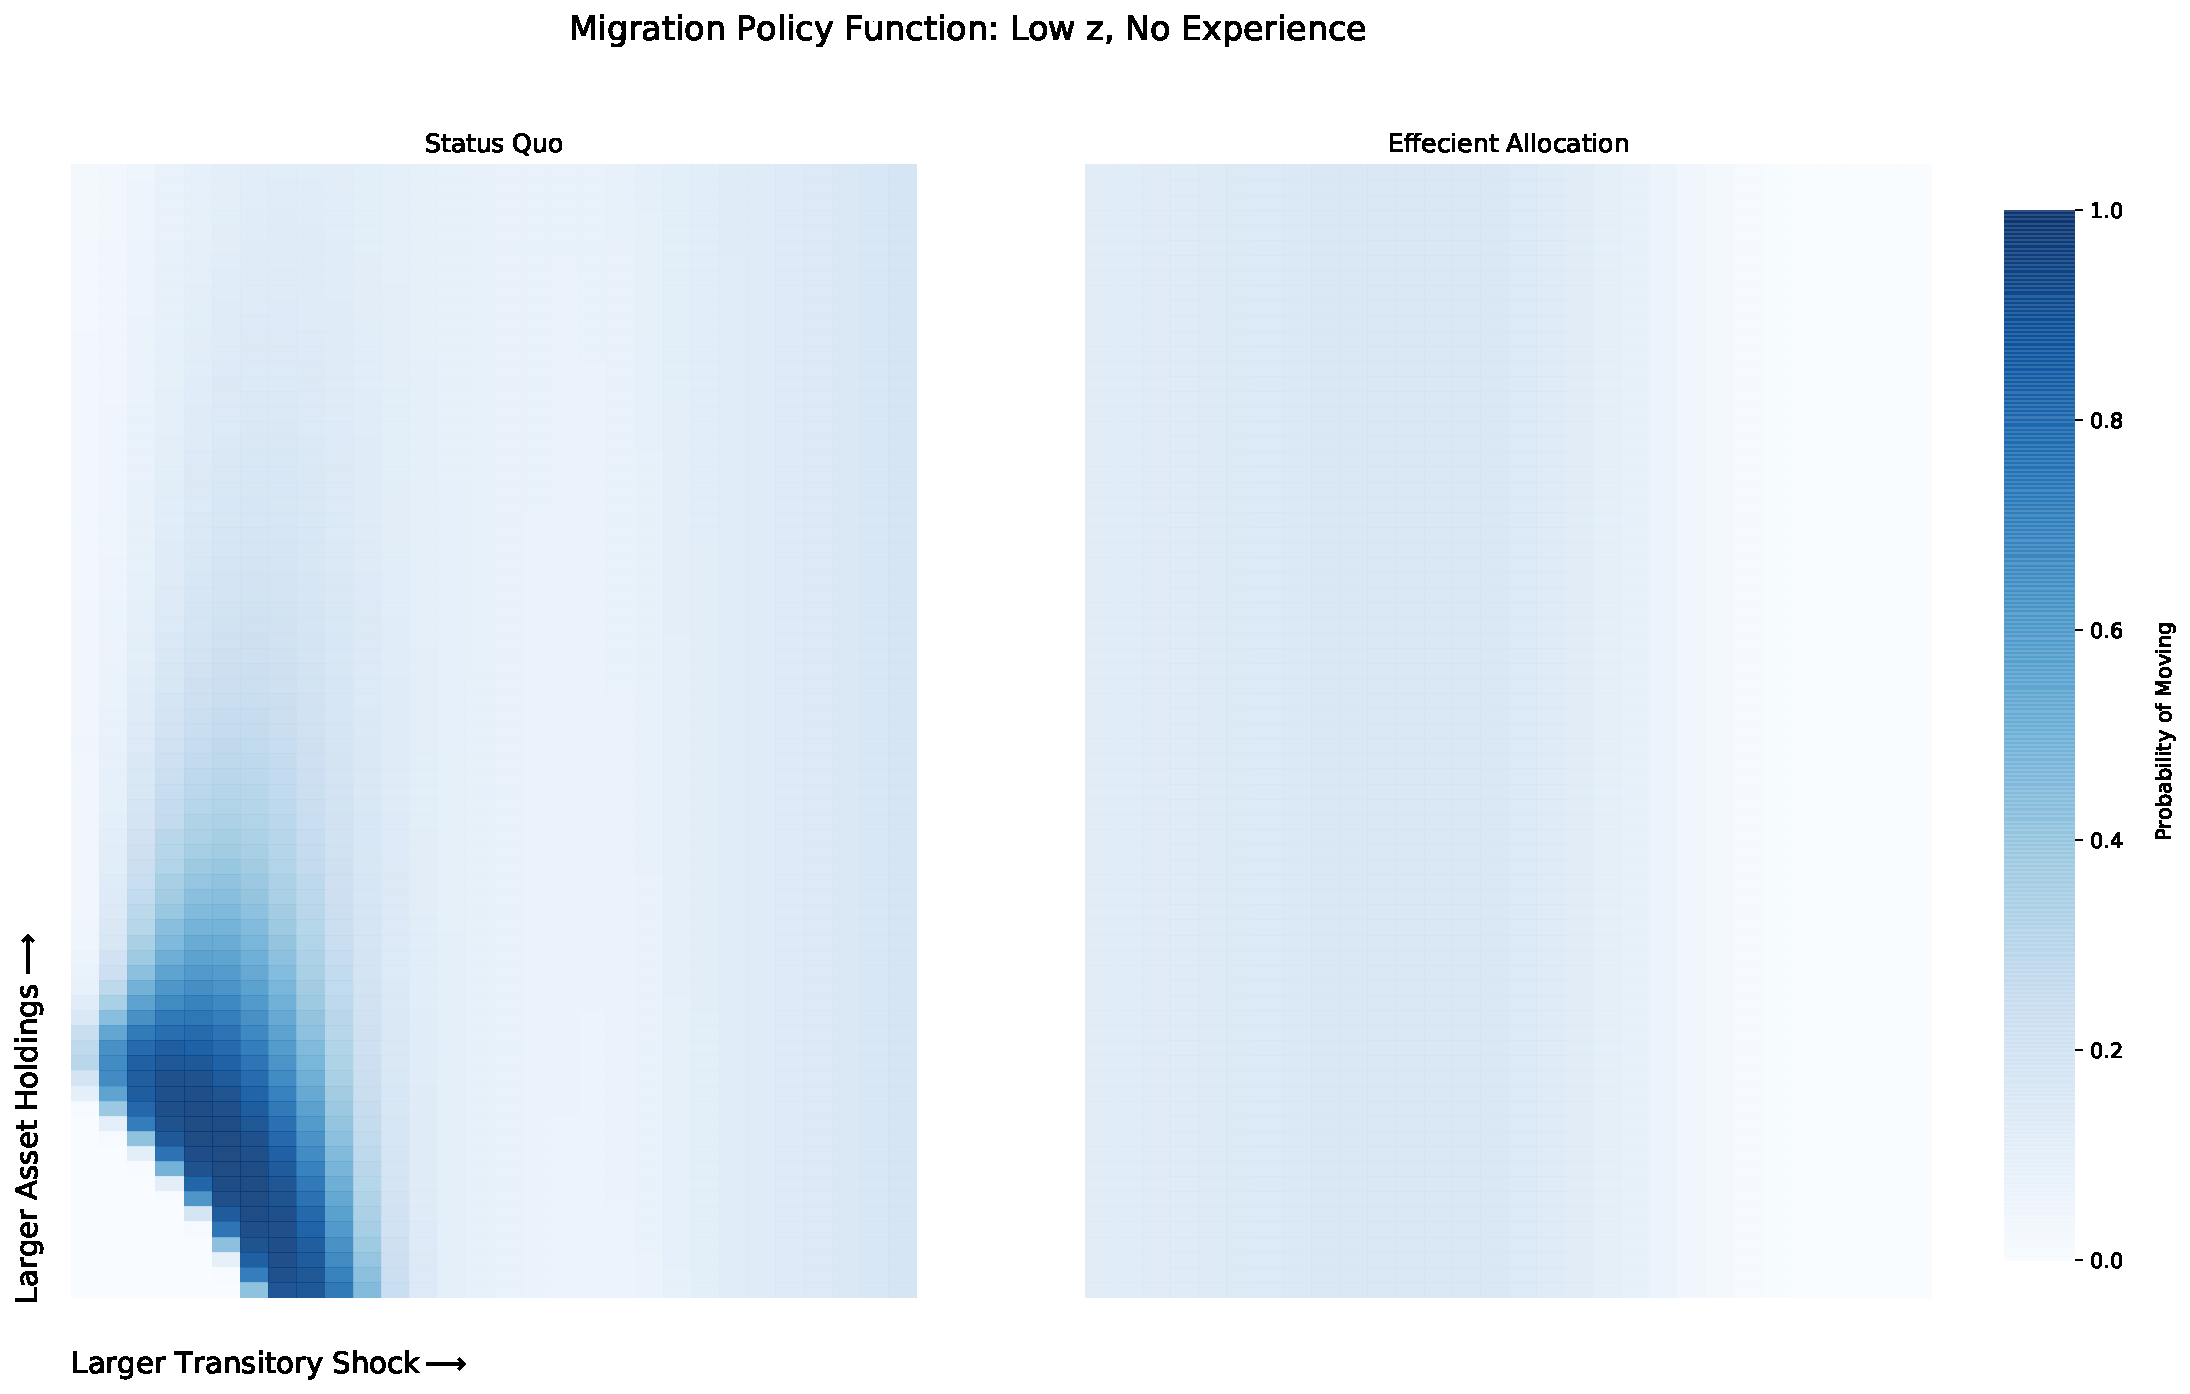
\includegraphics[scale = 0.50]{../figures/effecient_migration_policy_low_z_both.pdf}}
\textbf{\caption{Migration Probabilities: Baseline vs. Efficient Allocation}\label{fig:efficient_policy_function}}
\end{figure}

The interesting question is this: How much better can the planner do by changing how households migrate and move across rural and urban areas? The third column answers this question by computing the efficient allocation. Interestingly, the planner chooses an allocation that induces a smaller rural population, has less seasonal migration and a smaller, but non-zero wage gap (as implied by the marginal product of labor) between rural and urban areas. The incremental welfare gains from changes in migration relative to the full insurance allocation are modest; about one and a half percent.

These results connect with the nature of those who move in the data and the calibrated model. Figure \ref{fig:efficient_policy_function} reproduces the plot of the seasonal migration policy function by transitory shock and asset holdings for low $z$ households on the left hand side; the right hand side are the migration probabilities chosen by the planner. In the competitive equilibrium, many migrants move out of ``desperation'' with low transitory shocks and low asset households scrambling to avoid the borrowing constraint in the lower left hand corner. From the planners perspective, these moves are socially wasteful as they are virtually eliminated. From the planners perspective, given these households insurance and keeping them in the rural area is the efficient thing to do. In aggregate, by eliminating these desperation moves, seasonal migration is lower than in the baseline allocation.

Three more paragraphs.

\textbf{1. Something about welfare and misallocation} Really what this says that from a welfare perspective, there is not much ``misallocation'' The real issue in the model is the lack of insurance and how this is behind the seemingly ease with which the BCM model pushed people to migrate. It is less about people not doing the right thing or constrained in their ability to do so.

\textbf{2. Discuss GE tax.} The issue here is that (i) it is clearly a second best policy as it pushes migration in the wrong direction, however, it is still welfare enhancing because the costs of distorting migration is small relative to the gains from providing insurance even indirectly via migration. So we see sizeable gains from the GE policy. And that is in fact what Table \ref{tb:effecient} shows. The big ``wedge'' is on insurance.

\textbf{3. discuss that the RCT is telling us about if we have too much or too little migration.} There is a linear map from RCT to a normative statement. One of the key things shaping ``too much'' migration is LATE vs. OLS and how it influences $\gamma$. When LATE = OLS, these desperation moves don't take place. So then, what I would call more traditional forces are taking place. Risk aversion prevents high productive guys from migrating as much along with the credit constraint. Then the planner has these guys move more and that is in fact what we see. This should be one paragraph.



\begin{table}[h!]
\small
\setlength {\tabcolsep}{1.5mm}
\renewcommand{\arraystretch}{2.30}
\refstepcounter{table}
\begin{center}\label{tb:effecient}
\begin{tabular}{l c c c }
\multicolumn{4}{c}{\normalsize \textbf{NOT for paper. BUT FOR YOU TO SEE, LATE = OLS vs. the Efficient Allocation}}\\
\hline
\hline
\footnotesize   & \footnotesize  \textbf{Baseline} & \footnotesize   \textbf{Full Insurance, Fix Migration} &  \footnotesize \textbf{Efficient Allocation} \\
\cmidrule(lr){2-2} \cmidrule(lr){3-3} \cmidrule(lr){4-4}
\footnotesize  Rural Population  & 60.0  & 60.0   & 56.9      \\
\footnotesize  Seasonal Migration & 42.5   & 42.5 & 52.6 \\
\footnotesize  Wage Gap  & 1.88  & 1.88  & 1.67     \\
\footnotesize Welfare Gain & --- & 43.2 & 44.37 \\
\hline
\end{tabular}
\parbox[c]{6.75in}{\vspace{.1cm}
{\footnotesize \textbf{Note:} }}
\end{center}
\end{table}


\newpage

\bibliography{./bib/migration_refs}

\newpage

\appendix

\section{Cutoffs, Migration Probabilities, and Expected Utility}\label{appendix:migration_probs}




\end{onehalfspacing}
\end{document} 